% !TEX program = lualatex
%==============================================================================
%  The Contrast-Source Volume Integral Equation, FFT Acceleration,
%  and the Seismic Grid T-Matrix.
%
%  Self-contained LuaLaTeX source. Compile with:
%      latexmk -lualatex ContrastSourceVIE.tex
%==============================================================================
\documentclass[11pt,a4paper]{article}

% --- LuaLaTeX font handling -------------------------------------------------
\usepackage{fontspec}
\setmainfont{Latin Modern Roman}

% --- Mathematics ------------------------------------------------------------
\usepackage{amsmath}
\usepackage{amssymb}
\usepackage{mathtools}

% --- Layout and typography --------------------------------------------------
\usepackage[margin=1in]{geometry}
\usepackage{microtype}
\usepackage{xcolor}
\usepackage{booktabs}

% --- Graphics ---------------------------------------------------------------
\usepackage{tikz}
\usetikzlibrary{arrows.meta, positioning}

% --- Hyperlinks -------------------------------------------------------------
\usepackage[colorlinks=true,
            linkcolor=blue!55!black,
            citecolor=blue!55!black,
            urlcolor=blue!55!black]{hyperref}
\hypersetup{
  pdftitle={The Contrast-Source Volume Integral Equation, FFT Acceleration, and the Seismic Grid T-Matrix},
  pdfauthor={Tod Nestor}
}

% --- Macros -----------------------------------------------------------------
\newcommand{\rd}{\mathrm{d}}
\newcommand{\ii}{\mathrm{i}}
\newcommand{\vr}{\mathbf{r}}
\newcommand{\uinc}{u^{\mathrm{inc}}}
\newcommand{\Gop}{\mathsf{G}}
\newcommand{\norm}[1]{\lVert #1 \rVert}

\title{\bfseries The Contrast-Source Volume Integral Equation,
FFT Acceleration, and the Seismic Grid T-Matrix\\[4pt]
\large Background, methods, and references for the discrete-cell scattering programme}
\author{Tod Nestor}
\date{16 June 2026}

\begin{document}
\maketitle

\begin{abstract}
This note collects the methodological background and the primary literature for the
discrete-cell scattering programme: the volume integral equation in its contrast-source form,
the inversion framework that grew from it, the fast-Fourier-transform acceleration that makes
it tractable in three dimensions, and its seismological realisation as a grid T-matrix. The
contrast-source idea of van den Berg and Abubakar recasts scattering and inversion in terms of
an induced source on the heterogeneity rather than the total field. The CG-FFT, adaptive
integral, and precorrected-FFT methods reduce the dense integral operator to a Toeplitz
convolution evaluated by FFT. In seismology, Jakobsen and collaborators built forward
modelling and waveform inversion directly on the Lippmann-Schwinger T-matrix, with
renormalised scattering series for strong contrast and distorted-Born iterative T-matrix
inversion. The closing section places the present cubic-cell T-matrix codebase within that
lineage.
\end{abstract}

\bigskip
\noindent\textbf{Companion series.}\enspace{\small\itshape One of a companion series on elastic
multiple scattering from cubic heterogeneities on a depth-stratified background, the T-matrix
programme $T=T_0(I-G_0T_0)^{-1}$: \textbf{(I)}~the stratified inter-site propagator, the
same-depth convergence theory, the SH and P/SV traction kernels, interplane side scattering and
the first-shell near stencil (\texttt{EwaldIntraPlanePropagator}); \textbf{(II)}~the
contrast-source volume integral equation and the CG-FFT / seismic grid T-matrix lineage
(\texttt{ContrastSourceVIE}); \textbf{(III)}~the directional partial-wave sweep matvec and the
Krylov multiple-scattering solve (\texttt{DirectionalSweepSolver}); with the empirical companion
\texttt{RQ1\_Planar\_Decomposition\_Proposal}. This is note~(II).}

\tableofcontents
\bigskip

%==============================================================================
\section{The volume integral equation and the contrast source}
%==============================================================================

Let a heterogeneity occupy a bounded domain $D$ embedded in a known background with Green's
operator $G_0$. Writing the total field as incident plus scattered, the field on $D$ obeys the
Lippmann-Schwinger volume integral equation,
\begin{equation}
\label{eq:ls}
u(\vr)=\uinc(\vr)+\int_D G_0(\vr,\vr')\,\chi(\vr')\,u(\vr')\,\rd V', \qquad \vr\in D,
\end{equation}
where $\chi$ is the \emph{contrast} (the local deviation of the medium from the background; for
the scalar wave problem $\chi\propto k^2-k_0^2$, for elastodynamics the density-and-modulus
contrast operator $\delta L$). The scattered field at receivers $S$ is the radiation of the
same induced quantity,
\begin{equation}
\label{eq:data}
u^{\mathrm{sc}}(\vr)=\int_D G_0(\vr,\vr')\,\chi(\vr')\,u(\vr')\,\rd V', \qquad \vr\in S .
\end{equation}

\paragraph{The contrast source.} Following van den Berg and Kleinman \cite{vdBKleinman1997},
introduce the \emph{contrast source} (the induced polarisation, or equivalent current)
\begin{equation}
w(\vr)=\chi(\vr)\,u(\vr), \qquad \vr\in D .
\end{equation}
The integral equation \eqref{eq:ls} and the data relation \eqref{eq:data} then split into a
\emph{state (object) equation} on $D$ and a \emph{data equation} on $S$,
\begin{equation}
\label{eq:cs}
w=\chi\,\uinc+\chi\,\Gop_D\, w \quad\text{on } D,
\qquad\qquad
f=\Gop_S\, w \quad\text{on } S,
\end{equation}
where $\Gop_D$ and $\Gop_S$ are the background Green's operator mapping a source on $D$ to the
field on $D$ and on $S$ respectively, and $f=u^{\mathrm{sc}}|_S$ is the measured data. The whole
nonlinearity of scattering now sits in the single product $\chi\,\Gop_D w$.

\begin{figure}[h]
\centering
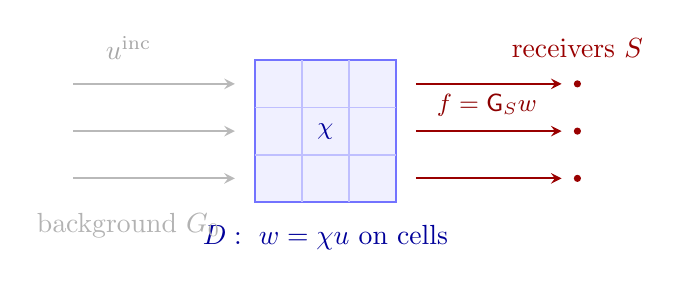
\begin{tikzpicture}[>=stealth, line width=0.7pt]
  \draw[fill=blue!6, draw=blue!55] (-0.9,-0.9) rectangle (0.9,0.9);
  \foreach \x in {-0.3,0.3} \draw[blue!25] (\x,-0.9)--(\x,0.9);
  \foreach \y in {-0.3,0.3} \draw[blue!25] (-0.9,\y)--(0.9,\y);
  \node[blue!60!black] at (0,0) {\small $\chi$};
  \node[blue!60!black] at (0,-1.35) {$D:\ w=\chi u$ on cells};
  \foreach \y in {-0.6,0,0.6} \draw[->, gray!55] (-3.2,\y)--(-1.15,\y);
  \node[gray!70] at (-2.5,1.05) {$\uinc$};
  \node[gray!60] at (-2.5,-1.2) {background $G_0$};
  \foreach \y in {-0.6,0,0.6} \draw[->, red!60!black] (1.15,\y)--(3.0,\y);
  \foreach \y in {-0.6,0,0.6} \fill[red!60!black] (3.2,\y) circle (1.3pt);
  \node[red!60!black] at (3.2,1.05) {receivers $S$};
  \node[red!55!black] at (2.05,0.33) {\small $f=\Gop_S w$};
\end{tikzpicture}
\caption{The volume integral equation in contrast-source form. The incident field $\uinc$
induces a contrast source $w=\chi u$ on the discretised heterogeneity $D$; the data $f$ are its
radiation through the background operator $\Gop_S$. The state equation couples the cells of $D$
through $\Gop_D$.}
\end{figure}

%==============================================================================
\section{Contrast source inversion}
%==============================================================================

The contrast-source split is the basis of the \emph{contrast source inversion} (CSI) method of
van den Berg and Abubakar \cite{vdBKleinman1997,vdBBroekhovenAbubakar1999,vdBAbubakar2001}. The
inverse problem is to recover $\chi$ from multi-experiment data $\{f_j\}$. CSI treats the
contrast $\chi$ and the contrast sources $\{w_j\}$ (one per illumination $j$) as
\emph{independent} unknowns and minimises a two-term normalised cost functional,
\begin{equation}
\label{eq:csi}
F(\chi,\{w_j\})=
\frac{\sum_j \norm{f_j-\Gop_S w_j}_S^2}{\sum_j \norm{f_j}_S^2}
\;+\;
\frac{\sum_j \norm{\chi\,\uinc_j-w_j+\chi\,\Gop_D w_j}_D^2}{\sum_j \norm{\chi\,\uinc_j}_D^2},
\end{equation}
the \emph{data error} plus the \emph{state error}. Minimisation alternates: with $\chi$ fixed,
each $w_j$ is updated by one conjugate-gradient step on \eqref{eq:csi}; with the $w_j$ fixed,
$\chi$ follows in closed form because $F$ is quadratic in $\chi$. The decisive feature is that
\emph{no forward problem is solved at any iteration}: the expensive operator inversion of
classical Born or Newton schemes is replaced by cheap gradient updates that drive the state
error to zero only as the iteration converges.

\paragraph{Regularisation.} Robustness to noise is obtained without a hand-tuned weight by the
multiplicatively regularised variant, MR-CSI, in which a weighted total-variation factor
multiplies \eqref{eq:csi} and adapts each iteration, preserving edges while suppressing noise
\cite{AbubakarvdBMallorqui2002}. CSI and MR-CSI have been carried across acoustic,
electromagnetic, and elastic settings, in two and three dimensions, including finite-difference
contrast-source variants for inhomogeneous backgrounds \cite{AbubakarHuvdBHabashy2008}; the
book of van den Berg \cite{vdB2021} is the comprehensive reference.

%==============================================================================
\section{FFT acceleration of the integral operator}
%==============================================================================

Every forward application of \eqref{eq:ls} or \eqref{eq:cs} requires the operator product
$\Gop_D w$, a discrete convolution of the background Green's function against the contrast
source over $D$. On a regular grid this operator is \emph{block-Toeplitz}, because
$G_0(\vr,\vr')$ depends only on $\vr-\vr'$, so the product is a convolution evaluated by the
fast Fourier transform in $O(N\log N)$ rather than the $O(N^2)$ of a dense matrix-vector
product. Paired with a Krylov solver (conjugate gradient, BiCGStab, GMRES), this is the
\emph{CG-FFT} method \cite{SarkarArvasRao1986}. The three-dimensional \emph{weak form} of
Zwamborn and van den Berg \cite{ZwambornvdB1992} tests and expands the equation so that the
singular kernel is integrated correctly while the Toeplitz structure, hence the FFT, is
retained.

For geometries that do not fall on a single regular grid, the same FFT speed is recovered by
projecting the interactions onto an auxiliary regular grid and correcting the near field
directly. This is the \emph{adaptive integral method} (AIM) of Bleszynski, Bleszynski, and
Jaroszewicz \cite{BleszynskiAIM1996} and the \emph{precorrected-FFT} (pFFT) method of Phillips
and White \cite{PhillipsWhite1997}. Both decompose the operator into a smooth far part, carried
by FFT on the auxiliary grid, and a sparse near part, computed and corrected in real space.
They are the FFT-based cousins of the fast multipole method, which instead accelerates the far
field through multipole expansions.

\begin{table}[h]
\centering
\renewcommand{\arraystretch}{1.25}
\begin{tabular}{@{}llll@{}}
\toprule
Method & Mesh & Far field via & Near field \\
\midrule
CG-FFT & regular grid & FFT (Toeplitz convolution) & exact on grid \\
AIM & arbitrary & FFT on auxiliary grid (moment match) & direct correction \\
pFFT & arbitrary & FFT on auxiliary grid (precorrection) & direct precorrection \\
FMM & arbitrary & multipole expansions & direct \\
\bottomrule
\end{tabular}
\caption{FFT-based and multipole accelerations of the dense integral operator. The first three
reduce the matrix-vector product to $O(N\log N)$ by exploiting grid translation invariance; all
treat the near field separately from the smooth far field.}
\end{table}

%==============================================================================
\section{The seismic grid T-matrix}
%==============================================================================

In seismology the same volume integral equation is most often written through the
\emph{T-matrix}. Let $V$ be the scattering potential (the perturbation operator of the
heterogeneity relative to the background $G_0$). The medium T-matrix resums the multiple
scattering of the whole object,
\begin{equation}
\label{eq:Tmatrix}
T=V\,(I-G_0 V)^{-1}, \qquad G=G_0+G_0\,T\,G_0,
\end{equation}
so that the Born series $T=V+VG_0V+VG_0VG_0V+\cdots$ is its weak-contrast expansion. Discretised
on a grid of cells, $V$ is block-diagonal (local) and $G_0$ is the background propagator; this
is exactly the discrete-cell programme. The elastic T-matrix for a flaw or inclusion dates to
Gubernatis, Domany, and Krumhansl \cite{GubernatisDomanyKrumhansl1977}, and Jakobsen and
collaborators built seismic forward modelling and inversion directly on \eqref{eq:Tmatrix}:
the T-matrix for effective-medium and rock-physics modelling \cite{JakobsenHudsonJohansen2003},
acoustic forward modelling on a grid \cite{Jakobsen2012}, and frequency-domain full-waveform
inversion by direct iterative T-matrix methods \cite{JakobsenUrsin2015}.

\paragraph{Strong contrast.} The Born series in \eqref{eq:Tmatrix} converges only when
$\norm{G_0 V}<1$, that is for weak contrast. For strong velocity contrasts the series must be
resummed. Jakobsen and Wu \cite{JakobsenWu2016} introduced a renormalised scattering series
that converges where the bare series diverges; the convergent Born series of Osnabrugge,
Leedumrongwatthanakun, and Vellekoop \cite{Osnabrugge2016} achieves the same end by
preconditioning the Lippmann-Schwinger equation with tuned absorption. Either way the
regular-grid Toeplitz structure of $G_0$, hence the FFT acceleration of Section~3, is preserved.

\paragraph{Inversion.} The T-matrix yields the Fr\'echet derivatives of the data with respect
to the contrast in closed form, which is the basis of the distorted-Born iterative T-matrix
(DBIT) inversion of Jakobsen and Ursin \cite{JakobsenUrsin2015}: a sequence of linearised
updates of $V$ about an evolving background, each reusing the same T-matrix machinery. This is
the seismological sibling of the contrast source inversion of Section~2; both avoid a full
forward solve per iteration, CSI by carrying the contrast sources as unknowns, DBIT by the
analytic T-matrix sensitivities.

%==============================================================================
\section{Placement of the present programme}
%==============================================================================

The cubic-cell T-matrix codebase is a specific, physically derived instance of this lineage.
Its global solve $T=T_0\,(I-G_0 T_0)^{-1}$ is the Foldy-Lax form of \eqref{eq:Tmatrix}, with the
bare per-cell contrast $V$ replaced by the single-cell T-matrix $T_0$ that already resums the
intra-cell scattering. Three choices distinguish it from the generic voxel volume integral
equation:

\begin{itemize}
\item \textbf{An analytic cell T-matrix.} $T_0$ is computed in closed form, from the cube
Eshelby tensor with the $r=0$ delta-function correction up to the 27-component Galerkin
representation under $O_h$ symmetry, rather than approximated by a point or piecewise-constant
contrast. The self-term singularity of the volume integral equation is thereby resolved inside
$T_0$.
\item \textbf{A layered background.} $G_0$ is the stratified (Kennett) propagator, not a
homogeneous whole-space Green's function, so the depth structure of the medium is carried
exactly while only the lateral contrast is discretised.
\item \textbf{FFT-accelerated Foldy-Lax.} The inter-cell coupling on the regular cubic grid is
block-Toeplitz and is applied by FFT inside a GMRES solve, exactly the CG-FFT acceleration of
Section~3.
\end{itemize}

In the language of this note, the programme is a contrast-source volume integral equation with
an analytic, physically exact cell T-matrix, an FFT-accelerated forward operator, and a layered
background, placed squarely in the seismic grid T-matrix tradition of Gubernatis and of Jakobsen
while contributing the closed-form cubic-cell scatterer.

%==============================================================================
\bibliographystyle{plain}
\bibliography{ContrastSourceVIE}

\end{document}
